\subsection{BSDF Path Integrator}

For this exercise, we implement a BSDF path integrator that samples
outgoing directions according to the BSDF instead of uniformly
sampling the hemisphere.

\lstinputlisting[
    language=C++,
    firstline=34,
    lastline=66,
    firstnumber=34,
    caption={BSDF path integrator}
]{../../assignments/integrators/bsdfpath.cpp}

Figure~\ref{fig:bsdf-comparison} compares the results of the
simple path integrator and the BSDF path integrator.

\begin{figure}[htbp]
    \centering
    \begin{minipage}{0.48\textwidth}
        \centering
        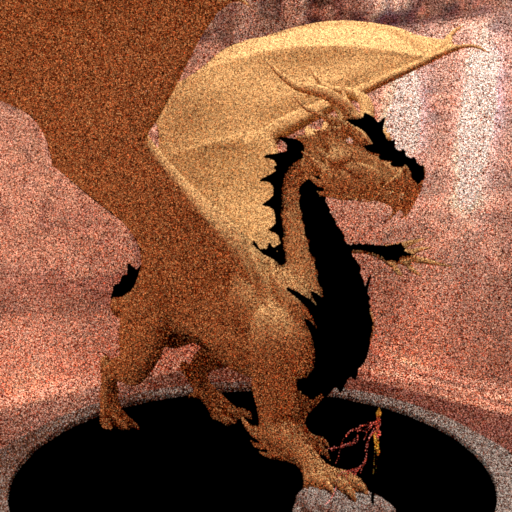
\includegraphics[width=\linewidth]{pictures/dragon-path.png}
        \small (a) Simple path integrator
    \end{minipage}
    \hfill
    \begin{minipage}{0.48\textwidth}
        \centering
        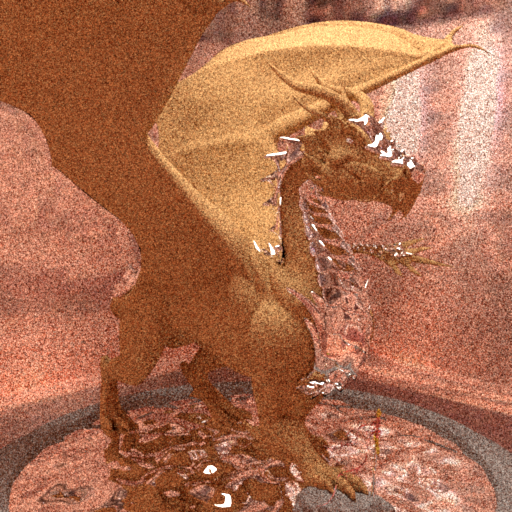
\includegraphics[width=\linewidth]{pictures/dragon-bsdfpath.png}
        \small (b) BSDF path integrator
    \end{minipage}
    \caption{Comparison of uniform hemisphere sampling and BSDF sampling.}
    \label{fig:bsdf-comparison}
\end{figure}

\paragraph{Why do we see this difference?}

With the simple path integrator, we sample directions uniformly over
the hemisphere. For an ideal mirror, the BSDF is nonzero only in the
perfect reflection direction. Since we sample from a continuous
distribution, the probability of choosing this exact direction is zero.

Moreover, the mirror BSDF is a delta distribution, and its
\texttt{eval()} method returns zero even if we somehow happen to sample
the correct direction. As a result, mirror surfaces appear black.

The BSDF path integrator avoids this problem by sampling directions
directly from the BSDF. For mirror surfaces, this means choosing the
reflection direction deterministically and obtaining the corresponding
contribution through \texttt{sample()}, rather than \texttt{eval()}.